\documentclass[tikz,border=0pt]{standalone}
\usepackage{xcolor}
\usetikzlibrary{calc}
% Palette: Sam_Comm_final.png by eye, and the drones and raiders.
\definecolor{ink}{HTML}{3B2340}
\definecolor{sky}{HTML}{EFC46A}
\definecolor{skyhi}{HTML}{F5DA92}
\definecolor{skylow}{HTML}{E9B060}
\definecolor{cloud}{HTML}{F2D58A}
\definecolor{paper}{HTML}{FBEFD0}
\definecolor{cream}{HTML}{FFF6E0}
\definecolor{white}{HTML}{FFFFFF}
\definecolor{wallA}{HTML}{E88A73}
\definecolor{wallB}{HTML}{EE9F7E}
\definecolor{wallC}{HTML}{E47A7E}
\definecolor{wallD}{HTML}{F0B07E}
\definecolor{wallE}{HTML}{D9765F}
\definecolor{wallF}{HTML}{E99A8A}
\definecolor{greenA}{HTML}{8DBB7E}
\definecolor{greenB}{HTML}{6FA77A}
\definecolor{greenC}{HTML}{A9C97F}
\definecolor{greenD}{HTML}{5E9C6A}
\definecolor{greenE}{HTML}{4A8060}
\definecolor{sage}{HTML}{9DB98A}
\definecolor{sagedark}{HTML}{6F8F66}
\definecolor{sagelight}{HTML}{C2D6A6}
\definecolor{window}{HTML}{F6E7A0}
\definecolor{windark}{HTML}{8C5A64}
\definecolor{metal}{HTML}{8D9A93}
\definecolor{metaldark}{HTML}{5E6B66}
\definecolor{metallight}{HTML}{B9C4BC}
\definecolor{wood}{HTML}{B9835A}
\definecolor{wooddark}{HTML}{8C5A3C}
\definecolor{woodlight}{HTML}{D9A66F}
\definecolor{stone}{HTML}{E7C9A0}
\definecolor{stonedark}{HTML}{C9A47E}
\definecolor{concrete}{HTML}{D8C3A4}
\definecolor{concretedark}{HTML}{B8A084}
\definecolor{asphalt}{HTML}{8E7A86}
\definecolor{asphaltdark}{HTML}{6E5C68}
\definecolor{roadline}{HTML}{F6E7A0}
\definecolor{kerb}{HTML}{D8B48C}
\definecolor{red}{HTML}{E0483E}
\definecolor{redlight}{HTML}{F27A6A}
\definecolor{gold}{HTML}{FFB000}
\definecolor{goldlight}{HTML}{FFD54F}
\definecolor{teal}{HTML}{4FA3A0}
\definecolor{tealdark}{HTML}{3C8582}
\definecolor{magenta}{HTML}{FF2E88}
\definecolor{cyan}{HTML}{13CFE3}
\definecolor{violet}{HTML}{8A5BD6}
\definecolor{orange}{HTML}{F2803A}
\definecolor{pink}{HTML}{F48FB1}
\definecolor{glow}{HTML}{4FE6E0}
\definecolor{glowhi}{HTML}{C8FFF9}
\definecolor{hot}{HTML}{FF6A1A}
\definecolor{hothi}{HTML}{FFD07A}
\definecolor{armour}{HTML}{7E7A86}
\definecolor{armourdark}{HTML}{5A5466}
\definecolor{armourlight}{HTML}{A8A2B0}
\definecolor{wasp}{HTML}{E0A82E}
\definecolor{waspdark}{HTML}{B07E1A}
\definecolor{moth}{HTML}{F2E6C8}
\definecolor{mothdark}{HTML}{D2C09A}
\definecolor{hornet}{HTML}{3C8582}
\definecolor{hornetdark}{HTML}{2C6260}
\definecolor{warden}{HTML}{E47A7E}
\definecolor{wardendark}{HTML}{B85A62}
\definecolor{tick}{HTML}{8DBB7E}
\definecolor{tickdark}{HTML}{5E8A5A}
\definecolor{strider}{HTML}{D9765F}
\definecolor{striderdark}{HTML}{A8543F}
\definecolor{jacket}{HTML}{6FA77A}
\definecolor{jacketb}{HTML}{4FA3A0}
\definecolor{jacketc}{HTML}{E88A73}
\definecolor{jacketd}{HTML}{F0B07E}
\definecolor{skin}{HTML}{F2C49A}
\definecolor{skinb}{HTML}{C98C6A}
\definecolor{skinc}{HTML}{8C5A3C}
\definecolor{hair}{HTML}{3B2340}
\definecolor{goo}{HTML}{B6E35A}
\definecolor{goodark}{HTML}{7FB23A}
\newcommand{\Ink}{1.8pt}
\tikzset{inked/.style={draw=ink, line width=\Ink, line join=round, line cap=round}}
\begin{document}
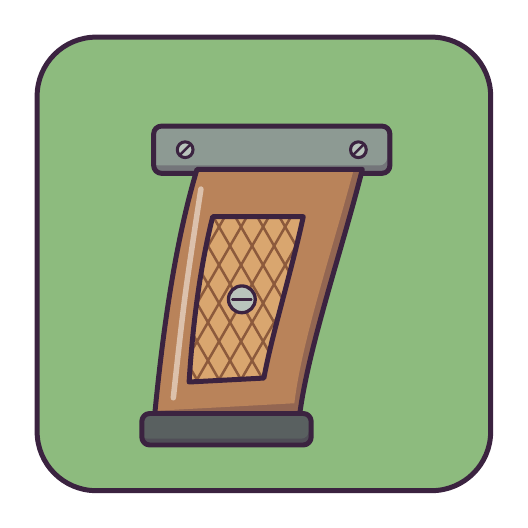
\begin{tikzpicture}
\clip (0,0) rectangle (6,6);
\fill[greenA] [rounded corners=0.75cm] (0.12,0.12) rectangle (5.88,5.88);
\begin{scope}\clip [rounded corners=0.75cm] (0.12,0.12) rectangle (5.88,5.88);
\begin{scope}\clip[rounded corners=0.1cm] (1.6,4.15) rectangle (4.6,4.75);
\fill[metal!70!ink,rounded corners=0.1cm] (1.6,4.15) rectangle (4.6,4.75);
\fill[metal,rounded corners=0.1cm, shift={(-0.035,0.1)}] (1.6,4.15) rectangle (4.6,4.75);
\end{scope}
\draw[inked,rounded corners=0.1cm] (1.6,4.15) rectangle (4.6,4.75);
\filldraw[inked,fill=metallight,line width=1.1pt] (2,4.45) circle (0.1);
\draw[ink, line width=0.9pt, line cap=round] (1.945,4.395) -- (2.055,4.505);
\filldraw[inked,fill=metallight,line width=1.1pt] (4.2,4.45) circle (0.1);
\draw[ink, line width=0.9pt, line cap=round] (4.145,4.395) -- (4.255,4.505);
\begin{scope}\clip (2.15,4.2) -- (4.25,4.2) .. controls (4.0,3.2) and (3.55,1.9) .. (3.45,1.05) -- (1.6,0.95) .. controls (1.7,2.0) and (1.85,3.2) .. (2.15,4.2) -- cycle;
\fill[wood!70!ink] (2.15,4.2) -- (4.25,4.2) .. controls (4.0,3.2) and (3.55,1.9) .. (3.45,1.05) -- (1.6,0.95) .. controls (1.7,2.0) and (1.85,3.2) .. (2.15,4.2) -- cycle;
\fill[wood, shift={(-0.063,0.18)}] (2.15,4.2) -- (4.25,4.2) .. controls (4.0,3.2) and (3.55,1.9) .. (3.45,1.05) -- (1.6,0.95) .. controls (1.7,2.0) and (1.85,3.2) .. (2.15,4.2) -- cycle;
\end{scope}
\draw[inked] (2.15,4.2) -- (4.25,4.2) .. controls (4.0,3.2) and (3.55,1.9) .. (3.45,1.05) -- (1.6,0.95) .. controls (1.7,2.0) and (1.85,3.2) .. (2.15,4.2) -- cycle;
\fill[woodlight] (2.35,3.6) -- (3.5,3.6) .. controls (3.35,2.9) and (3.1,2.1) .. (3.0,1.55) -- (2.05,1.5) .. controls (2.1,2.3) and (2.2,3.0) .. (2.35,3.6) -- cycle;
\begin{scope}\clip (2.35,3.6) -- (3.5,3.6) .. controls (3.35,2.9) and (3.1,2.1) .. (3.0,1.55) -- (2.05,1.5) .. controls (2.1,2.3) and (2.2,3.0) .. (2.35,3.6) -- cycle;
\draw[wooddark, line width=0.9pt] (-0.28,1.2) -- (1.22,3.8);
\draw[wooddark, line width=0.9pt] (-0.28,3.8) -- (1.22,1.2);
\draw[wooddark, line width=0.9pt] (0,1.2) -- (1.5,3.8);
\draw[wooddark, line width=0.9pt] (0,3.8) -- (1.5,1.2);
\draw[wooddark, line width=0.9pt] (0.28,1.2) -- (1.78,3.8);
\draw[wooddark, line width=0.9pt] (0.28,3.8) -- (1.78,1.2);
\draw[wooddark, line width=0.9pt] (0.56,1.2) -- (2.06,3.8);
\draw[wooddark, line width=0.9pt] (0.56,3.8) -- (2.06,1.2);
\draw[wooddark, line width=0.9pt] (0.84,1.2) -- (2.34,3.8);
\draw[wooddark, line width=0.9pt] (0.84,3.8) -- (2.34,1.2);
\draw[wooddark, line width=0.9pt] (1.12,1.2) -- (2.62,3.8);
\draw[wooddark, line width=0.9pt] (1.12,3.8) -- (2.62,1.2);
\draw[wooddark, line width=0.9pt] (1.4,1.2) -- (2.9,3.8);
\draw[wooddark, line width=0.9pt] (1.4,3.8) -- (2.9,1.2);
\draw[wooddark, line width=0.9pt] (1.68,1.2) -- (3.18,3.8);
\draw[wooddark, line width=0.9pt] (1.68,3.8) -- (3.18,1.2);
\draw[wooddark, line width=0.9pt] (1.96,1.2) -- (3.46,3.8);
\draw[wooddark, line width=0.9pt] (1.96,3.8) -- (3.46,1.2);
\draw[wooddark, line width=0.9pt] (2.24,1.2) -- (3.74,3.8);
\draw[wooddark, line width=0.9pt] (2.24,3.8) -- (3.74,1.2);
\draw[wooddark, line width=0.9pt] (2.52,1.2) -- (4.02,3.8);
\draw[wooddark, line width=0.9pt] (2.52,3.8) -- (4.02,1.2);
\draw[wooddark, line width=0.9pt] (2.8,1.2) -- (4.3,3.8);
\draw[wooddark, line width=0.9pt] (2.8,3.8) -- (4.3,1.2);
\draw[wooddark, line width=0.9pt] (3.08,1.2) -- (4.58,3.8);
\draw[wooddark, line width=0.9pt] (3.08,3.8) -- (4.58,1.2);
\draw[wooddark, line width=0.9pt] (3.36,1.2) -- (4.86,3.8);
\draw[wooddark, line width=0.9pt] (3.36,3.8) -- (4.86,1.2);
\draw[wooddark, line width=0.9pt] (3.64,1.2) -- (5.14,3.8);
\draw[wooddark, line width=0.9pt] (3.64,3.8) -- (5.14,1.2);
\draw[wooddark, line width=0.9pt] (3.92,1.2) -- (5.42,3.8);
\draw[wooddark, line width=0.9pt] (3.92,3.8) -- (5.42,1.2);
\end{scope}
\draw[inked] (2.35,3.6) -- (3.5,3.6) .. controls (3.35,2.9) and (3.1,2.1) .. (3.0,1.55) -- (2.05,1.5) .. controls (2.1,2.3) and (2.2,3.0) .. (2.35,3.6) -- cycle;
\draw[white, line width=2pt, line cap=round, line join=round, opacity=0.5] plot[smooth, tension=0.6] coordinates {(2.2,3.95) (2,2.6) (1.85,1.3)};
\begin{scope}\clip[rounded corners=0.1cm] (1.45,0.7) rectangle (3.6,1.1);
\fill[metaldark!85!ink!70!ink,rounded corners=0.1cm] (1.45,0.7) rectangle (3.6,1.1);
\fill[metaldark!85!ink,rounded corners=0.1cm, shift={(-0.028,0.08)}] (1.45,0.7) rectangle (3.6,1.1);
\end{scope}
\draw[inked,rounded corners=0.1cm] (1.45,0.7) rectangle (3.6,1.1);
\filldraw[inked,fill=metallight,line width=1.2pt] (2.72,2.55) circle (0.17);
\draw[ink, line width=1pt, line cap=round] (2.6,2.55) -- (2.84,2.55);
\end{scope}
\draw[inked] [rounded corners=0.75cm] (0.12,0.12) rectangle (5.88,5.88);
\end{tikzpicture}
\end{document}
